% ============================================================
%  05_giaodien.tex – Chương 5: Thiết kế giao diện
% ============================================================
\chapter{Thiết Kế Giao Diện}

\section{Định Hướng Thiết Kế}

Frontend sử dụng phong cách ấm, tươi và gần gũi với ngành hàng trái cây. Màu cam được dùng cho hành động chính; ảnh sản phẩm giữ vai trò trung tâm; bố cục card và khoảng trắng giúp người dùng quét nhanh danh sách. Giao diện quản trị ưu tiên mật độ thông tin, bảng dữ liệu và bộ lọc.

Các nguyên tắc chính gồm:

\begin{itemize}[leftmargin=2em, itemsep=4pt]
  \item \textbf{Nhất quán:} dùng chung header, footer, card sản phẩm, trạng thái và hệ thống màu.
  \item \textbf{Responsive:} lưới sản phẩm, form checkout và navigation thay đổi theo chiều rộng màn hình; mobile có bottom navigation.
  \item \textbf{Phản hồi:} các request có loading/error/empty state; thao tác giỏ hàng có toast; nút submit bị khóa trong lúc xử lý.
  \item \textbf{Giảm ma sát mua hàng:} giỏ được lưu lại, checkout chấp nhận khách vãng lai và phí giao hàng hiển thị trước khi đặt đơn.
  \item \textbf{Phân quyền:} menu và route quản trị chỉ hiển thị khi người dùng có quyền tương ứng.
\end{itemize}

\section{Sơ Đồ Điều Hướng Frontend}

Luồng mua hàng chính được tổ chức ngắn gọn theo chuỗi: \textit{Trang chủ/Danh mục/Tìm kiếm} $\rightarrow$ \textit{Chi tiết sản phẩm hoặc hộp tự chọn} $\rightarrow$ \textit{Giỏ hàng} $\rightarrow$ \textit{Checkout} $\rightarrow$ \textit{Xác nhận đơn}. Khách đã đăng nhập có thể đi tiếp tới lịch sử đơn; blog, liên hệ và chính sách là các nhánh nội dung độc lập từ thanh điều hướng chung. Cấu trúc này giữ hành động mua hàng trong tối đa vài bước rõ ràng và vẫn cho phép khám phá nội dung thương hiệu.

\section{Các Màn Hình Khách Hàng}

\begin{longtable}{@{}p{0.25\textwidth} p{0.24\textwidth} p{0.43\textwidth}@{}}
  \toprule
  \textbf{Màn hình} & \textbf{Đường dẫn} & \textbf{Chức năng} \\
  \midrule
  \endhead
  Trang chủ & \texttt{/} & Banner động, nhóm danh mục, sản phẩm nổi bật và nội dung thương hiệu. \\
  Danh sách sản phẩm & \texttt{/products} & Lưới sản phẩm, lọc, sắp xếp và điều hướng tới chi tiết. \\
  Chi tiết sản phẩm & \texttt{/products/:slug} & Ảnh, mô tả, biến thể, giá, số lượng, thành phần và thêm giỏ. \\
  Danh mục & \texttt{/categories/:slug} & Danh sách sản phẩm trong một danh mục động. \\
  Tìm kiếm & \texttt{/search} & Từ khóa, lọc danh mục/mức giá và trạng thái không có kết quả. \\
  Hộp tự chọn & \texttt{/custom-box/:slug} & Tạo cấu hình hộp theo lựa chọn thành phần và ngân sách. \\
  Giỏ hàng & \texttt{/cart} & Chọn dòng hàng, đổi số lượng, xóa và chuyển sang checkout. \\
  Checkout & \texttt{/checkout} & Người nhận, định vị, phí ship, mã khuyến mãi, tóm tắt và đặt đơn. \\
  Tài khoản & \texttt{/account} & Thông tin người dùng và điều hướng tới lịch sử đơn. \\
  Lịch sử đơn & \texttt{/order-history} & Danh sách đơn của khách đang đăng nhập và mã đơn hiển thị. \\
  Blog & \texttt{/blog/:id} & Danh sách và nội dung bài viết theo dữ liệu CMS. \\
  Trang tĩnh & \texttt{/about-us}, \texttt{/contact}, các policy & Giới thiệu, liên hệ, thanh toán, giao hàng và quyền riêng tư. \\
  \bottomrule
\end{longtable}

\section{Ảnh Chụp Giao Diện Từ Phiên Chạy Thử}

Các hình dưới đây được chụp trực tiếp tại \texttt{localhost:5173}. Bộ ảnh được chọn theo hành trình sử dụng thay vì chụp mọi route: sáu màn hình khách hàng bao quát khám phá--cấu hình--tư vấn--checkout và bốn màn hình quản trị bao quát KPI--catalog--đơn hàng--tồn kho. Dữ liệu catalog, giá, ảnh, giỏ hàng và KPI đều đến từ API của dự án, không phải mockup tĩnh.

\begin{figure}[H]
  \centering
  \begin{subfigure}[t]{0.49\textwidth}
    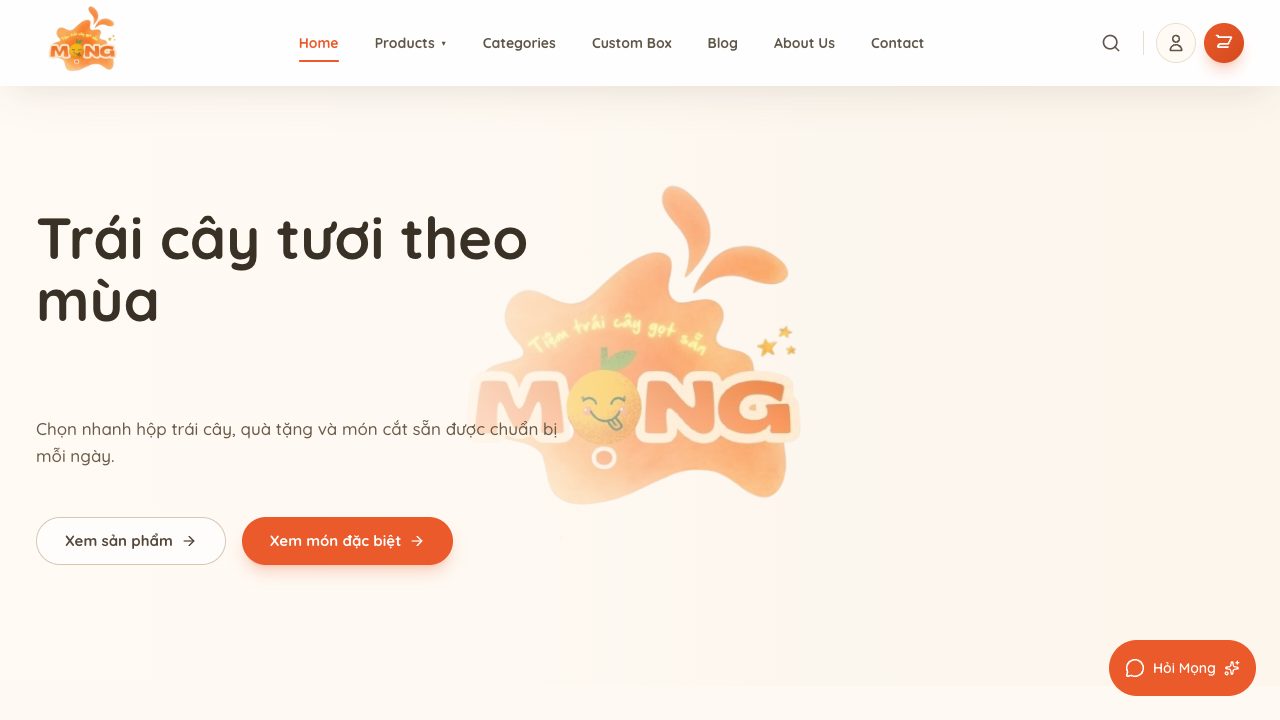
\includegraphics[width=\linewidth]{images/ui-home.png}
    \caption{Trang chủ và nhận diện thương hiệu}
  \end{subfigure}\hfill
  \begin{subfigure}[t]{0.49\textwidth}
    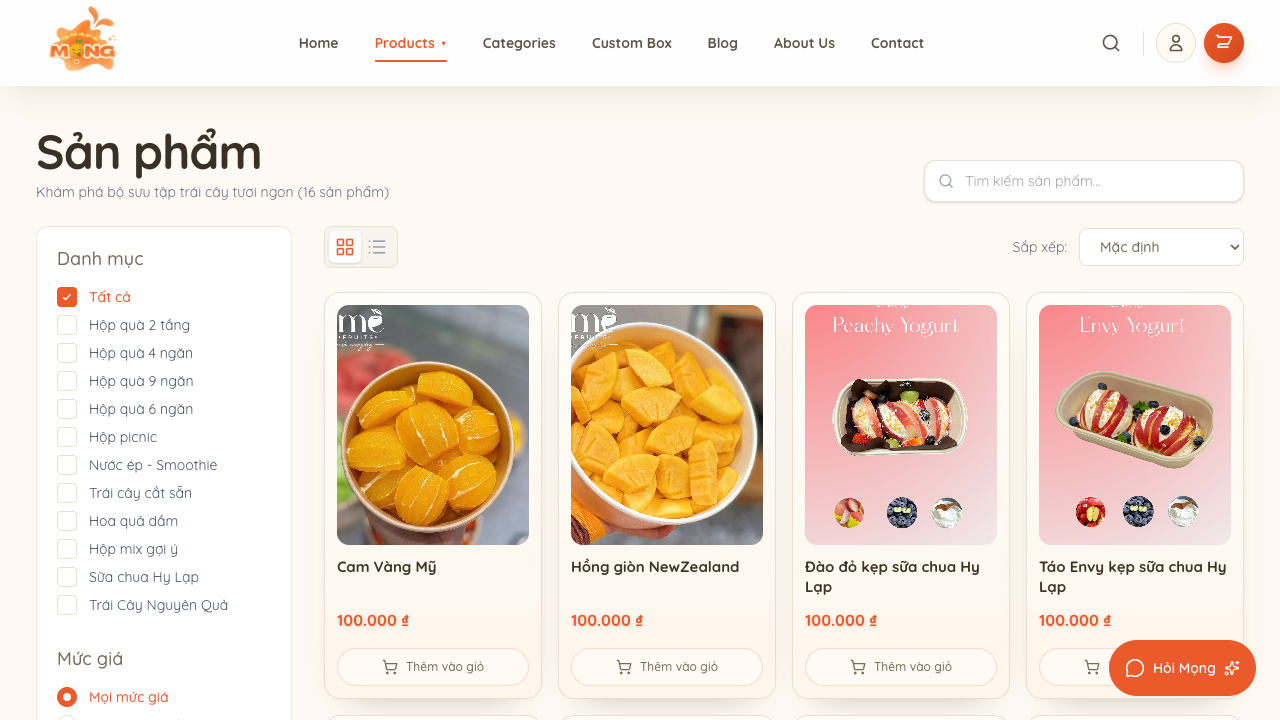
\includegraphics[width=\linewidth]{images/ui-products.png}
    \caption{Catalog và bộ lọc sản phẩm}
  \end{subfigure}
  \caption{Hai điểm vào chính của hành trình khám phá sản phẩm}
  \label{fig:ui-discovery}
\end{figure}

\begin{figure}[H]
  \centering
  \begin{subfigure}[t]{0.49\textwidth}
    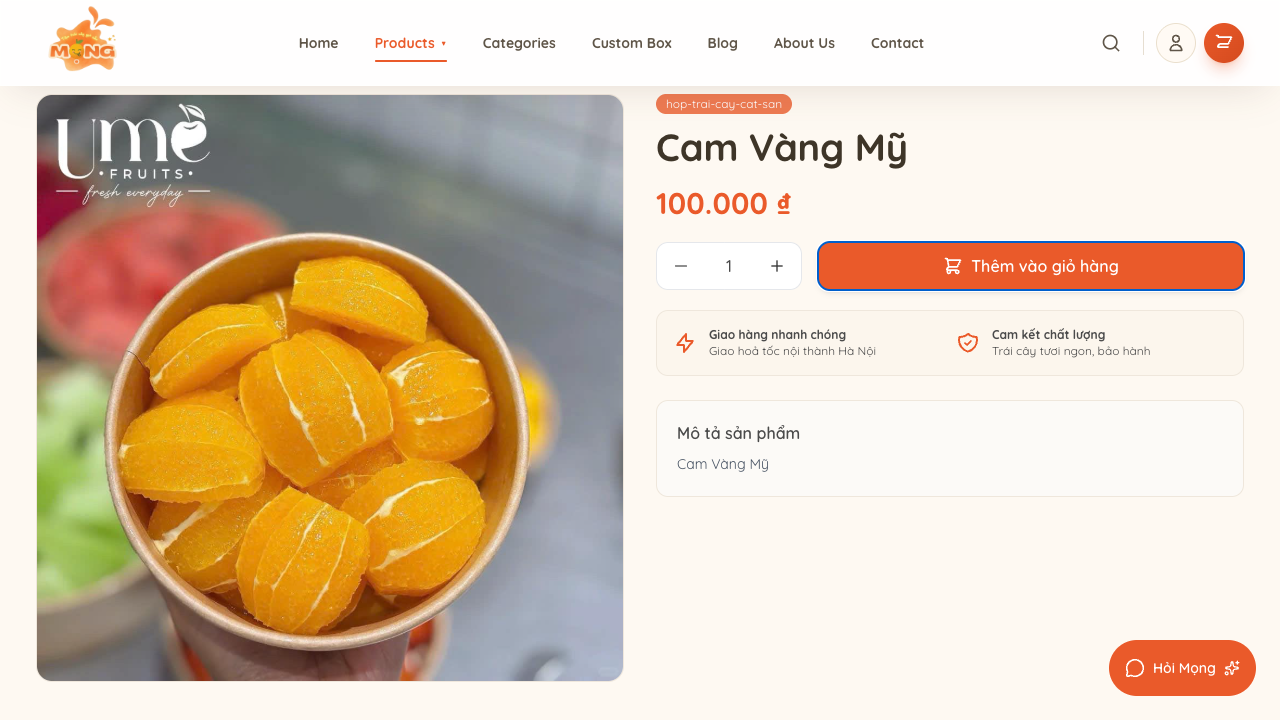
\includegraphics[width=\linewidth]{images/ui-product-detail.png}
    \caption{Chi tiết sản phẩm và biến thể}
  \end{subfigure}\hfill
  \begin{subfigure}[t]{0.49\textwidth}
    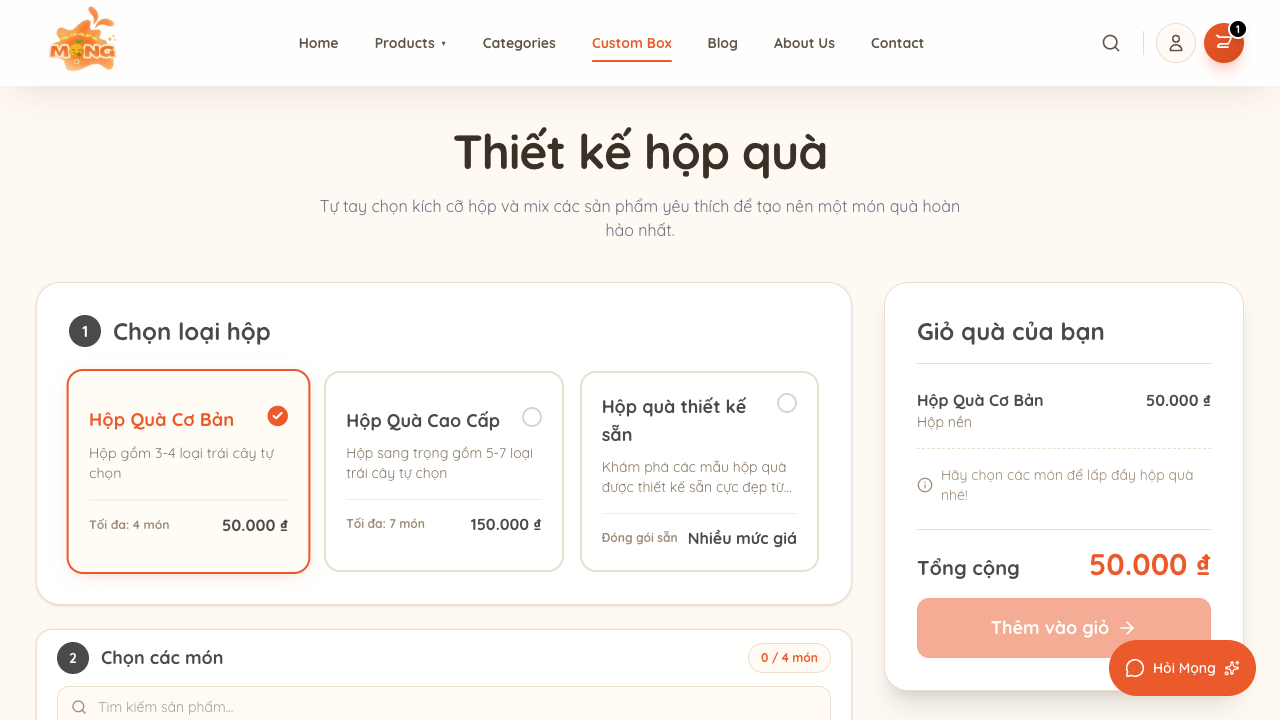
\includegraphics[width=\linewidth]{images/ui-custom-box.png}
    \caption{Tùy chọn thành phần hộp quà}
  \end{subfigure}
  \caption{Hai cách cấu hình sản phẩm trước khi thêm vào giỏ}
  \label{fig:ui-product-config}
\end{figure}

\begin{figure}[H]
  \centering
  \begin{subfigure}[t]{0.49\textwidth}
    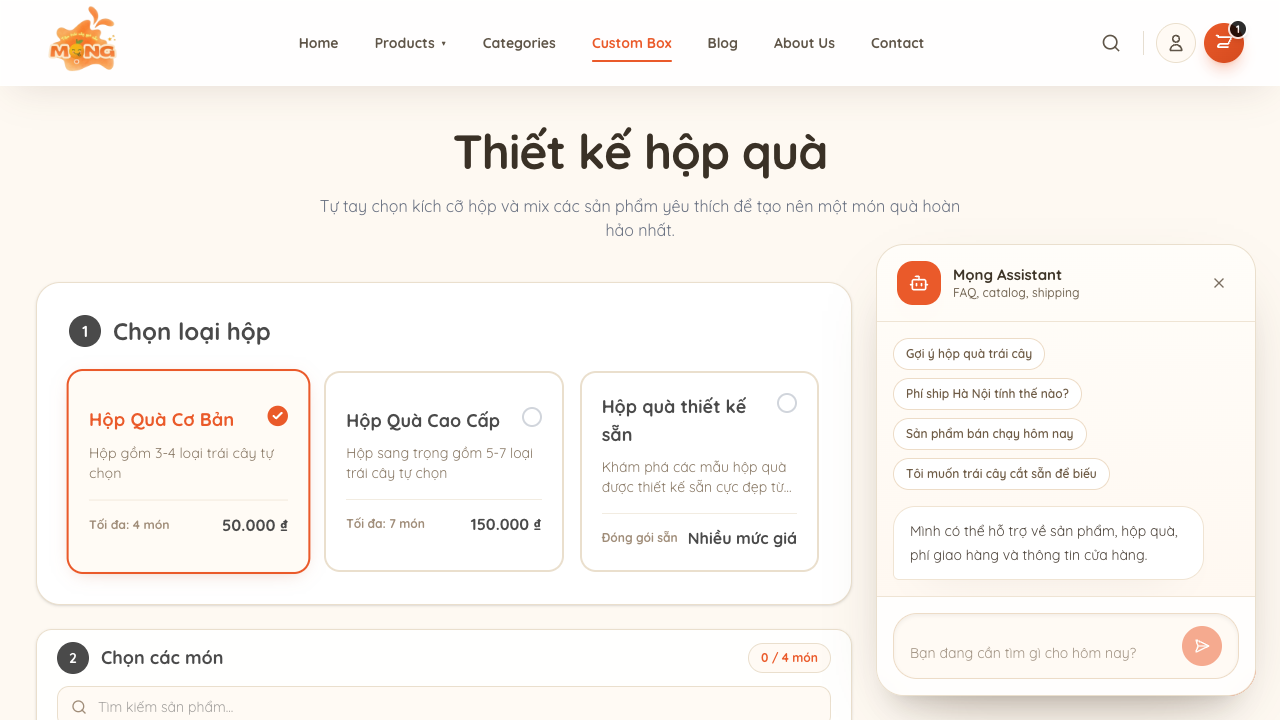
\includegraphics[width=\linewidth]{images/ui-chatbot.png}
    \caption{Chatbot tư vấn trong ngữ cảnh frontend}
  \end{subfigure}\hfill
  \begin{subfigure}[t]{0.49\textwidth}
    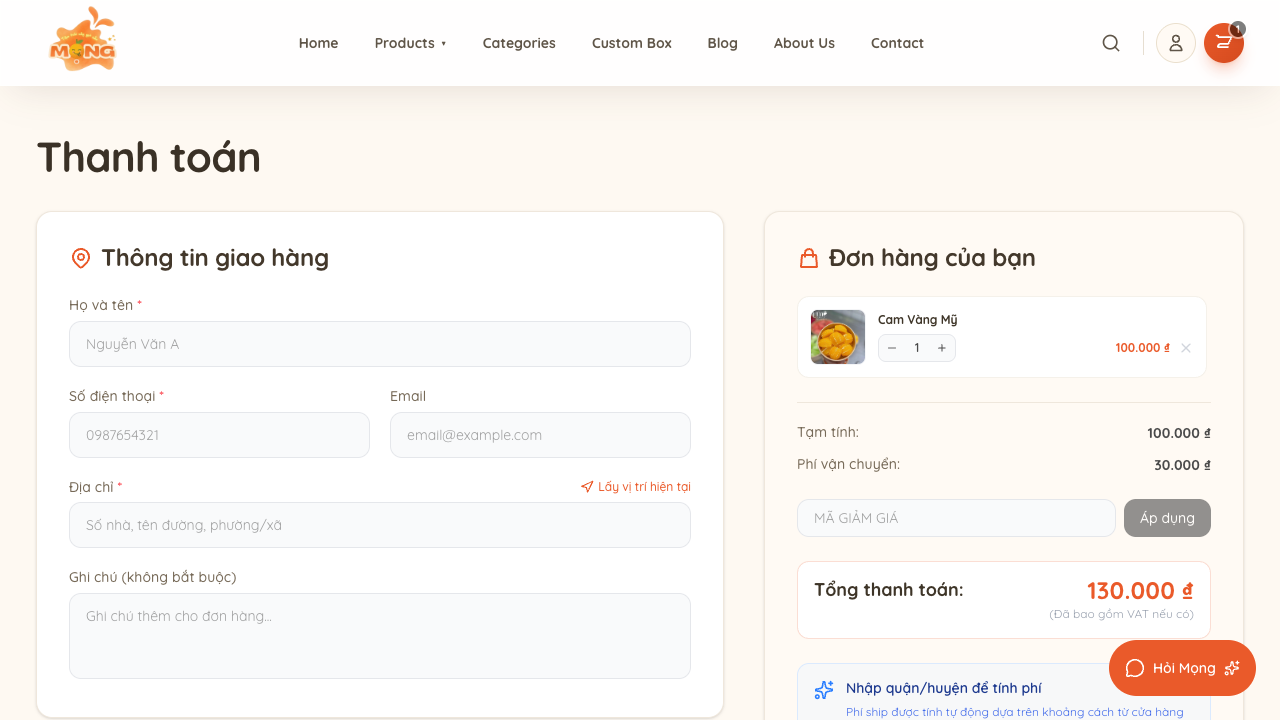
\includegraphics[width=\linewidth]{images/ui-checkout.png}
    \caption{Checkout và tóm tắt tổng đơn}
  \end{subfigure}
  \caption{Hỗ trợ quyết định mua và hoàn tất đơn hàng}
  \label{fig:ui-assist-checkout}
\end{figure}

\subsection{Trang sản phẩm và chi tiết}

Card sản phẩm gom ảnh, tên, giá và hành động mua. Trang chi tiết dùng route động theo slug, nhờ đó không cần tạo file riêng cho từng sản phẩm. Khi sản phẩm có nhiều biến thể, người dùng phải chọn biến thể trước khi thêm vào giỏ. Giao diện review và thao tác gửi điểm đã được loại bỏ; phần dưới trang tập trung vào mô tả, thành phần nguyên liệu và sản phẩm liên quan.

\subsection{Giỏ hàng và checkout}

Giỏ hàng cho phép chọn một phần sản phẩm để checkout. Tại trang checkout, số lượng vẫn có thể chỉnh; hệ thống tính subtotal, giảm giá, phí giao hàng và tổng. Người dùng có thể lấy tọa độ hiện tại để reverse geocode hoặc nhập địa chỉ thủ công. Phí ship được debounce khi địa chỉ thay đổi và có cách tính offline dự phòng cho các quận Hà Nội.

\subsection{Chatbot}

ChatbotWidget xuất hiện trên frontend dưới dạng nút nổi. Câu trả lời hỗ trợ Markdown và có thể kèm card gợi ý sản phẩm. UI cần phân biệt trạng thái đang gửi, lỗi giới hạn tần suất và phản hồi fallback để khách hiểu mức độ chắc chắn của thông tin.

Qua phiên chạy thử, bố cục khách hàng có thứ bậc thị giác rõ: hành động chính dùng màu cam, nội dung bán hàng dùng card và ảnh lớn, chatbot nổi ở góc nhưng không che nút checkout. Điểm nên cải thiện là thống nhất chiều cao ảnh sản phẩm, tăng tương phản một số chữ phụ và hiển thị rõ hơn nguồn tính phí giao hàng trước khi người dùng xác nhận.

\section{Khu Vực Quản Trị}

Quản trị được đặt dưới namespace \texttt{/admin}. \texttt{AdminLayout} cung cấp sidebar, header và vùng nội dung; \texttt{ProtectedRoute} yêu cầu đăng nhập; \texttt{RequirePermission} chặn các màn hình cần quyền cụ thể.

\begin{longtable}{@{}p{0.27\textwidth} p{0.26\textwidth} p{0.39\textwidth}@{}}
  \toprule
  \textbf{Nhóm quản trị} & \textbf{Route tiêu biểu} & \textbf{Nghiệp vụ} \\
  \midrule
  \endhead
  Dashboard & \texttt{/admin}, \texttt{/admin/finance} & KPI tổng quan, doanh thu, chi phí và lợi nhuận. \\
  Catalog & \texttt{/admin/products}, \texttt{/admin/categories} & CRUD sản phẩm, biến thể, ảnh và danh mục. \\
  Kho và nguyên liệu & \texttt{/admin/inventory}, \texttt{/admin/ingredients} & Mức tồn, giá vốn, loại nguyên liệu và công thức. \\
  Bán hàng & \texttt{/admin/orders}, \texttt{/admin/promotions} & Theo dõi đơn, trạng thái và điều kiện khuyến mãi. \\
  Khách hàng & \texttt{/admin/customers} & Hồ sơ khách hàng và lịch sử mua hàng. \\
  Nội dung & \texttt{/admin/banners}, \texttt{/admin/blog}, \texttt{/admin/media} & Banner, bài viết, danh mục blog và thư viện ảnh. \\
  Cấu hình & \texttt{/admin/settings/*}, \texttt{/admin/content/*} & Giao hàng, website, chính sách và FAQ chatbot. \\
  Vận hành hệ thống & \texttt{/admin/search}, \texttt{/admin/chatbot} & Trạng thái chỉ mục và câu hỏi chatbot chưa xử lý. \\
  Phân quyền & \texttt{/admin/users}, \texttt{/admin/roles} & Người dùng nội bộ, role và permission. \\
  \bottomrule
\end{longtable}

Các trang danh sách dùng chung \texttt{AdminListFilters} để tìm kiếm và lọc. Form tạo/sửa được tách thành route riêng. Trạng thái admin được chuẩn hóa bằng các component loading, error và empty để tránh mỗi trang tự định nghĩa cách hiển thị khác nhau.

\begin{figure}[H]
  \centering
  \begin{subfigure}[t]{0.49\textwidth}
    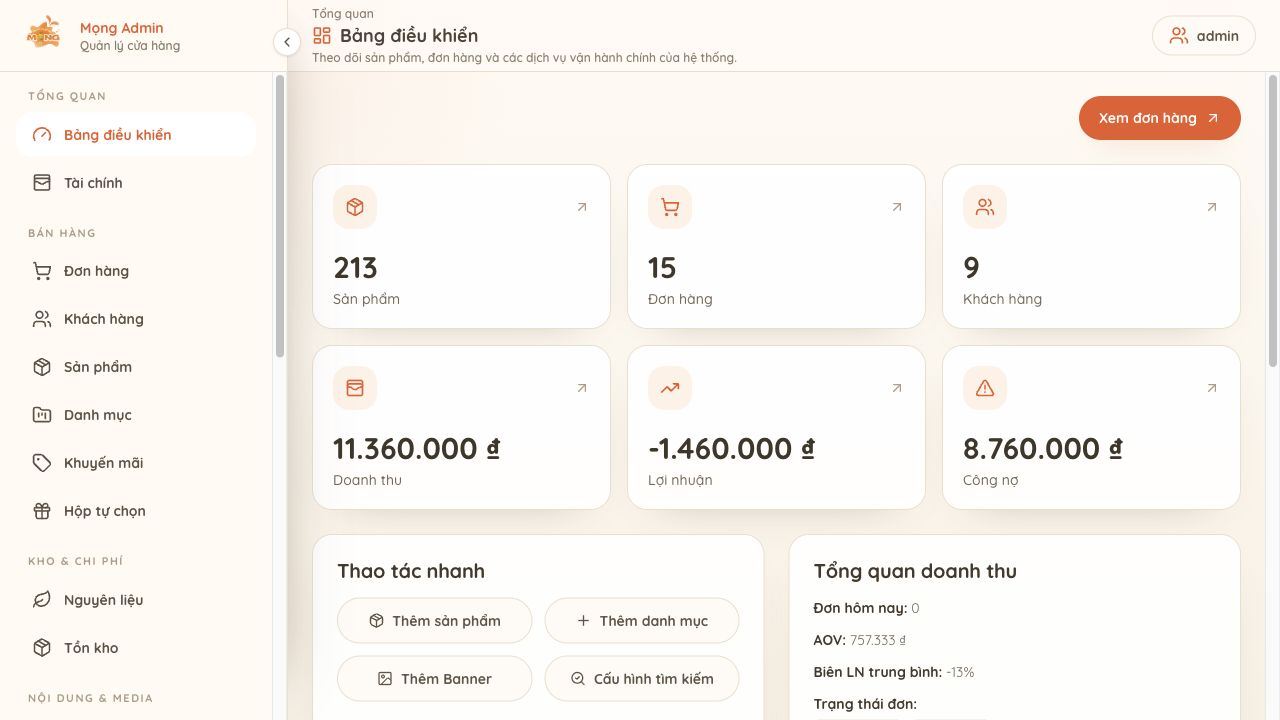
\includegraphics[width=\linewidth]{images/ui-admin-dashboard.png}
    \caption{Dashboard và KPI vận hành}
  \end{subfigure}\hfill
  \begin{subfigure}[t]{0.49\textwidth}
    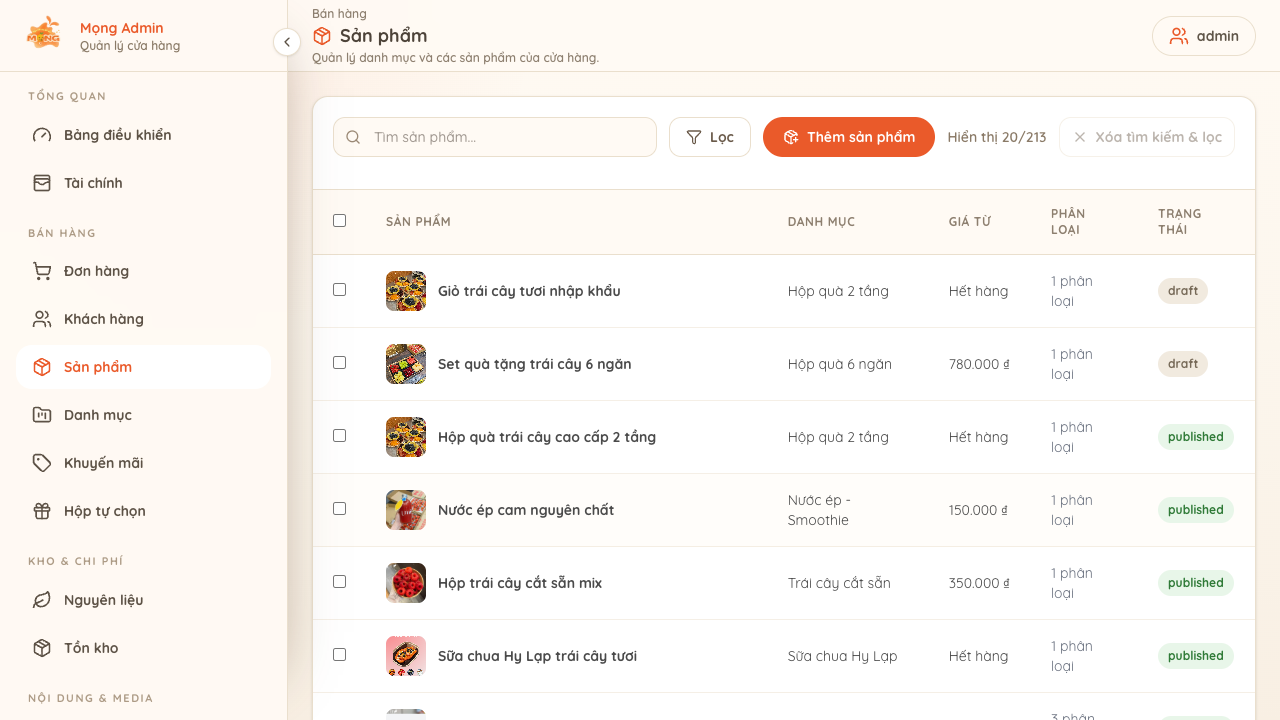
\includegraphics[width=\linewidth]{images/ui-admin-products.png}
    \caption{Danh sách sản phẩm quản trị}
  \end{subfigure}
  \caption{Tổng quan vận hành và quản trị catalog}
  \label{fig:ui-admin-overview}
\end{figure}

\begin{figure}[H]
  \centering
  \begin{subfigure}[t]{0.49\textwidth}
    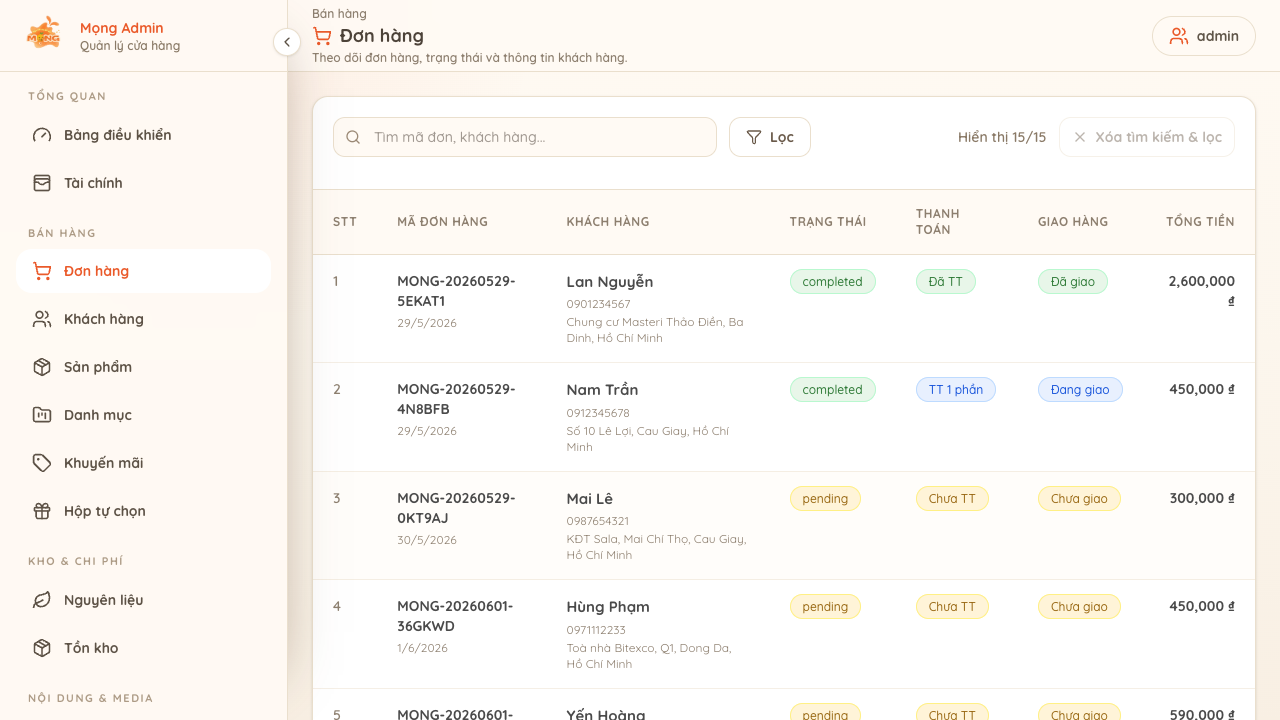
\includegraphics[width=\linewidth]{images/ui-admin-orders.png}
    \caption{Theo dõi đơn hàng và trạng thái}
  \end{subfigure}\hfill
  \begin{subfigure}[t]{0.49\textwidth}
    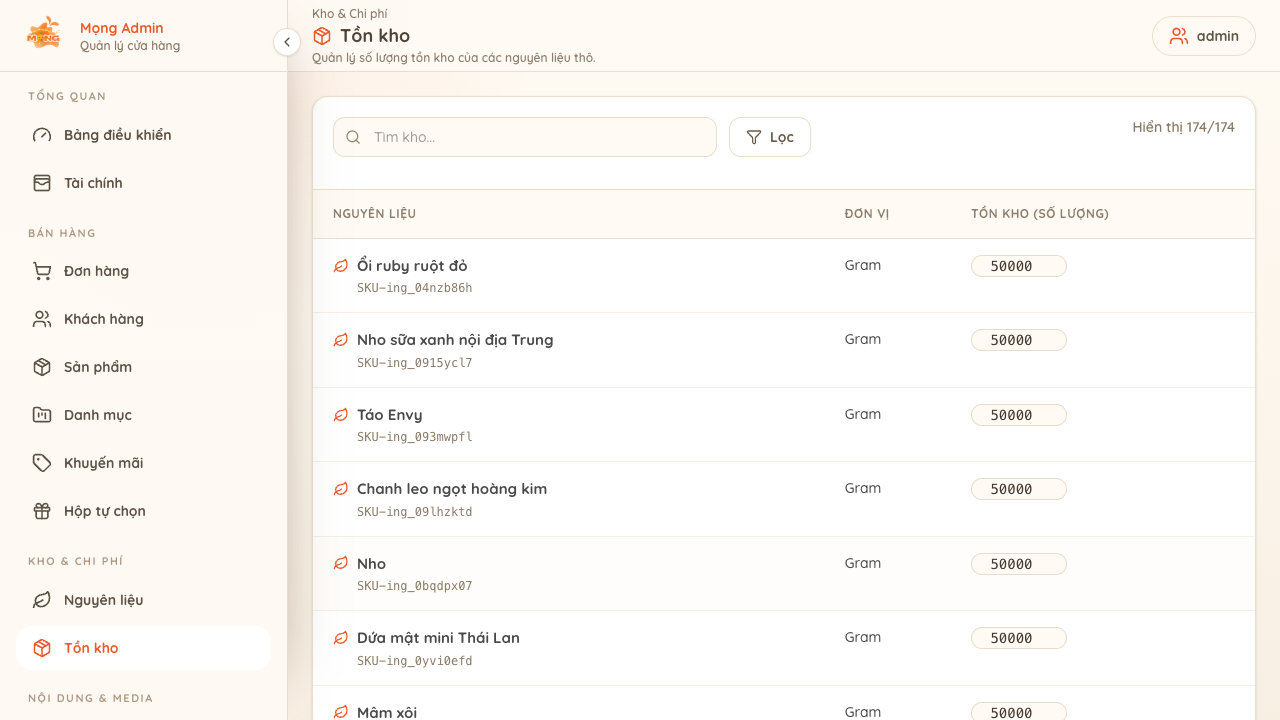
\includegraphics[width=\linewidth]{images/ui-admin-inventory.png}
    \caption{Mức tồn kho theo mặt hàng}
  \end{subfigure}
  \caption{Hai màn hình tác nghiệp bán hàng và kho}
  \label{fig:ui-admin-operations}
\end{figure}

Các bảng quản trị giữ bộ lọc và hành động ở vùng đầu trang, giúp nhân viên chuyển nhanh từ quan sát sang xử lý. Dashboard phù hợp để nhận biết xu hướng; trang đơn hàng cung cấp dữ liệu tác nghiệp; trang tồn kho hỗ trợ quyết định nhập hoặc điều chỉnh hàng. Cần tiếp tục chuẩn hóa tên trạng thái tiếng Việt, định dạng tiền và mật độ cột giữa các bảng để giảm thời gian làm quen.

\section{Khả Năng Tiếp Cận và Responsive}

Một số nền tảng tốt đã có như lazy loading route, bottom navigation trên mobile và nhãn trạng thái rõ ràng. Tuy nhiên, cần tiếp tục rà soát khả năng dùng bàn phím, focus khi mở modal, vùng chạm tối thiểu 44 px và thông báo động cho trình đọc màn hình. Đặc biệt, số lượng giỏ nên dùng \texttt{aria-live="polite"}; ảnh dưới màn hình đầu nên đặt \texttt{loading="lazy"}; trang sản phẩm nên bổ sung JSON-LD và metadata SEO.

\section{Đánh Giá Tính Nhất Quán}

Frontend và admin hiện cùng nằm trong một ứng dụng React nhưng phục vụ hai phong cách sử dụng khác nhau. Cách tổ chức này thuận tiện khi phát triển nhanh, song bundle và design system có thể trở nên lớn. Trong giai đoạn tiếp theo có thể tách admin thành workspace riêng hoặc chuyển các phần quản trị phù hợp sang Medusa Admin extensions, đồng thời chuẩn hóa màu, typography, component bảng và form dùng chung.
